\documentclass[a4paper, 12pt]{article}

% packages
\usepackage{amssymb}
\usepackage[fleqn]{mathtools}
\usepackage{tikz}
\usepackage{enumerate}
\usepackage{bussproofs}
\usepackage{xcolor}
\usepackage[margin=1.3cm]{geometry}
\usepackage{logicproof}
\usepackage{diagbox}
\usepackage{listings}
\usepackage{graphicx}
\usepackage{lstautogobble}
\usepackage{hyperref}
\usepackage{multirow}
\usepackage{tipa}
\usepackage{pgfplots}

% tikz libraries
\usetikzlibrary{
    decorations.pathreplacing,
    arrows,
    shapes.gates.logic.US,
    circuits.logic.US,
    calc,
    automata,
    positioning,
    intersections
}

\pgfplotsset{compat=1.16}

\pgfmathdeclarefunction{gauss}{2}{%
  \pgfmathparse{1/(#2*sqrt(2*pi))*exp(-((x-#1)^2)/(2*#2^2))}%
}

\allowdisplaybreaks % allow environments to break
\setlength\parindent{0pt} % no indent

% shorthand for verbatim
% this clashes with logicproof, so maybe fix this at some point?
\catcode`~=\active
\def~#1~{\texttt{#1}}

% code listing
\lstdefinestyle{main}{
    numberstyle=\tiny,
    breaklines=true,
    showspaces=false,
    showstringspaces=false,
    tabsize=2,
    numbers=left,
    basicstyle=\ttfamily,
    columns=fixed,
    fontadjust=true,
    basewidth=0.5em,
    autogobble,
    xleftmargin=3.0ex,
    mathescape=true
}
\newcommand{\dollar}{\mbox{\textdollar}} %
\lstset{style=main}

% augmented matrix
\makeatletter
\renewcommand*\env@matrix[1][*\c@MaxMatrixCols c]{%
\hskip -\arraycolsep
\let\@ifnextchar\new@ifnextchar
\array{#1}}
\makeatother

% ceiling / floor
\DeclarePairedDelimiter{\ceil}{\lceil}{\rceil}
\DeclarePairedDelimiter{\floor}{\lfloor}{\rfloor}

% custom commands
\newcommand{\indefint}[2]{\int #1 \, \mathrm{d}#2}
\newcommand{\defint}[4]{\int_{#1}^{#2} #3 \, \mathrm{d}#4}
\newcommand{\pdif}[2]{\frac{\partial #1}{\partial #2}}
\newcommand{\dif}[2]{\frac{\mathrm{d}#1}{\mathrm{d}#2}}
\newcommand{\limit}[2]{\raisebox{0.5ex}{\scalebox{0.8}{$\displaystyle{\lim_{#1 \to #2}}$}}}
\newcommand{\limitsup}[2]{\raisebox{0.5ex}{\scalebox{0.8}{$\displaystyle{\limsup_{#1 \to #2}}$}}}
\newcommand{\summation}[2]{\sum\limits_{#1}^{#2}}
\newcommand{\product}[2]{\prod\limits_{#1}^{#2}}
\newcommand{\intbracket}[3]{\left[#3\right]_{#1}^{#2}}
\newcommand{\laplace}{\mathcal{L}}
\newcommand{\fourier}{\mathcal{F}}
\newcommand{\mat}[1]{\boldsymbol{#1}}
\renewcommand{\vec}[1]{\boldsymbol{#1}}
\newcommand{\rowt}[1]{\begin{bmatrix}
    #1
\end{bmatrix}^\top}
\DeclareMathOperator*{\argmax}{argmax}
\DeclareMathOperator*{\argmin}{argmin}

\newcommand{\lto}[0]{\leadsto\ }

\newcommand{\ulsmash}[1]{\underline{\smash{#1}}}

\newcommand{\powerset}[0]{\wp}
\renewcommand{\emptyset}[0]{\varnothing}

\makeatletter
\newsavebox{\@brx}
\newcommand{\llangle}[1][]{\savebox{\@brx}{\(\m@th{#1\langle}\)}%
  \mathopen{\copy\@brx\kern-0.5\wd\@brx\usebox{\@brx}}}
\newcommand{\rrangle}[1][]{\savebox{\@brx}{\(\m@th{#1\rangle}\)}%
  \mathclose{\copy\@brx\kern-0.5\wd\@brx\usebox{\@brx}}}
\makeatother
\newcommand{\lla}{\llangle}
\newcommand{\rra}{\rrangle}
\newcommand{\la}{\langle}
\newcommand{\ra}{\rangle}
\newcommand{\crnr}[1]{\text{\textopencorner} #1 \text{\textcorner}}
\newcommand{\bnfsep}[0]{\ |\ }
\newcommand{\concsep}[0]{\ ||\ }

\newcommand{\axiom}[1]{\AxiomC{#1}}
\newcommand{\unary}[1]{\UnaryInfC{#1}}
\newcommand{\binary}[1]{\BinaryInfC{#1}}
\newcommand{\trinary}[1]{\TrinaryInfC{#1}}
\newcommand{\quaternary}[1]{\QuaternaryInfC{#1}}
\newcommand{\quinary}[1]{\QuinaryInfC{#1}}
\newcommand{\dproof}[0]{\DisplayProof}

\newcommand{\ttbs}{\char`\\}
\newcommand{\lrbt}[0]{\ \bullet\ }

% colours
\newcommand{\violet}[1]{\textcolor{violet}{#1}}
\newcommand{\blue}[1]{\textcolor{blue}{#1}}
\newcommand{\red}[1]{\textcolor{red}{#1}}
\newcommand{\teal}[1]{\textcolor{teal}{#1}}

% reasoning proofs
\usepackage{ltablex}
\usepackage{environ}
\keepXColumns
\NewEnviron{reasoning}{
    \begin{tabularx}{\textwidth}{rlX}
        \BODY
    \end{tabularx}
}
\newcommand{\proofline}[3]{$(#1)$ & $#2$ & \hfill #3 \smallskip \\}
\newcommand{\proofarbitrary}[1]{& take arbitrary $#1$ \smallskip \\}
\newcommand{\prooftext}[1]{\multicolumn{3}{l}{#1} \smallskip \\}
\newcommand{\proofmath}[3]{$#1$ & = $#2$ & \hfill #3 \smallskip \\}
\newcommand{\prooftherefore}[1]{& $\therefore #1$ \smallskip \\}
\newcommand{\proofbc}[0]{\prooftext{\textbf{Base Case}}}
\newcommand{\proofis}[0]{\prooftext{\textbf{Inductive Step}}}

% ER diagrams
\newcommand{\nattribute}[4]{
    \node[draw, state, inner sep=0cm, minimum size=0.2cm, label=#3:{#4}] (#1) at (#2) {};
}
\newcommand{\mattribute}[4]{
    \node[draw, state, accepting, inner sep=0cm, minimum size=0.2cm, label=#3:{#4}] (#1) at (#2) {};
}
\newcommand{\dattribute}[4]{
    \node[draw, state, dashed, inner sep=0cm, minimum size=0.2cm, label=#3:{#4}] (#1) at (#2) {};
}
\newcommand{\entity}[3]{
    \node[] (#1-c) at (#2) {#3};
    \node[inner sep=0cm] (#1-l) at ($(#1-c) + (-1, 0)$) {};
    \node[inner sep=0cm] (#1-r) at ($(#1-c) + (1, 0)$) {};
    \node[inner sep=0cm] (#1-u) at ($(#1-c) + (0, 0.5)$) {};
    \node[inner sep=0cm] (#1-d) at ($(#1-c) + (0, -0.5)$) {};
    \draw
    ($(#1-c) + (-1, 0.5)$) -- ($(#1-c) + (1, 0.5)$) -- ($(#1-c) + (1, -0.5)$) -- ($(#1-c) + (-1, -0.5)$) -- cycle;
}
\newcommand{\relationship}[3]{
    \node[] (#1-c) at (#2) {#3};
    \node[inner sep=0cm] (#1-l) at ($(#1-c) + (-1, 0)$) {};
    \node[inner sep=0cm] (#1-r) at ($(#1-c) + (1, 0)$) {};
    \node[inner sep=0cm] (#1-u) at ($(#1-c) + (0, 1)$) {};
    \node[inner sep=0cm] (#1-d) at ($(#1-c) + (0, -1)$) {};
    \draw
    ($(#1-c) + (-1, 0)$) -- ($(#1-c) + (0, 1)$) -- ($(#1-c) + (1, 0)$) -- ($(#1-c) + (0, -1)$) -- cycle;
}

% AVL Trees
\newcommand{\avltri}[4]{
    \draw ($(#1)$) -- ($(#1) + #4*(0.5, -1)$) -- ($(#1) + #4*(-0.5, -1)$) -- cycle;
    \node at ($(#1) + #4*(0, -1) + (0, 0.5)$) {#3};
    \node at ($(#1) + #4*(0, -1) + (0, -0.5)$) {#2};
}

% RB Trees
\tikzset{rbtr/.style={inner sep=2pt, circle, draw=black, fill=red}}
\tikzset{rbtb/.style={inner sep=2pt, circle, draw=black, fill=black}}

% actual document
\begin{document}
    \section*{CO220 - Software Engineering Design}
        \subsection*{8th October 2019}
            \subsubsection*{Cost of Change}
                \begin{center}
                    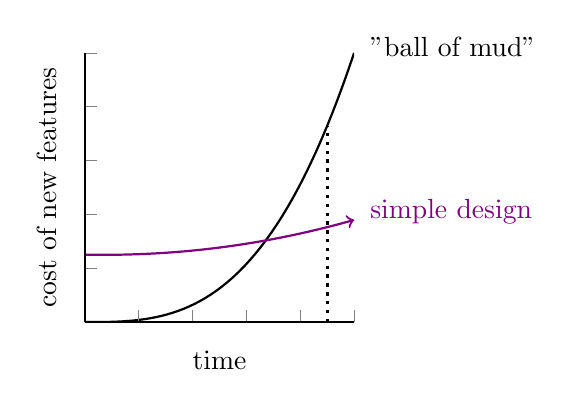
\begin{tikzpicture}
                        \begin{axis}[
                            axis on top=true,
                            axis line style=thick,
                            no markers, domain=0:10, samples=50,
                            axis lines*=left, xlabel={time}, ylabel={cost of new features},
                            height=5cm, width=5cm,
                            enlargelimits=false,
                            xticklabels={,,},
                            yticklabels={,,}
                        ]
                            \addplot[mark=none, black, very thick, dotted] coordinates {(9, 0) (9, 729)};
                            \addplot[thick] {\x^3};
                            \addplot[violet, thick, ->] {250+\x^1.75*ln(\x)};
                        \end{axis}
                        \node[anchor=west] at (3.5, 3.5) {"ball of mud"};
                        \node[anchor=west] at (3.5, 1.4) {\violet{simple design}};
                    \end{tikzpicture}
                \end{center}
                The "project heat death", denoted by the dotted line, is where the cost of adding new features outweighs the value gained by adding those features.
                Note that the initial cost of doing a simple design can be more expensive (since it requires more planning).
            \subsubsection*{Elements of Simple Design}
                This is arranged in a pyramid on the slides (since they "build up on each other") but I will write it as a list, starting from the bottom;
                \begin{enumerate}[1.]
                    \itemsep0em
                    \item \textbf{behaves correctly}
                        \medskip

                        It doesn't matter if the codebase is well structured, or the code is elegant if it doesn't do the right thing (is buggy, or isn't what the customer wanted).
                        \begin{itemize}
                            \itemsep0em
                            \item automated testing
                            \item test-driven development
                            \item mock objects
                        \end{itemize}
                    \item \textbf{minimises duplication}
                        \medskip

                        If something needs to be changed in the future, and it's in multiple places, it will have to be changed in all of those places which will take longer.
                        Additionally, it's also easy to miss, causing bugs.
                    \item \textbf{maximises clarity}
                        \medskip

                        Code should be easy to modify, such that the parts that need to be changed can be easily located.
                        Important especially if working with others.
                    \item \textbf{has fewer elements}
                        \medskip

                        Less important - we want to focus on the previous levels first, and don't want to lose the benefits by combining elements.
                \end{enumerate}
            \subsubsection*{Test-Driven Development / Behaviour Driven Development}
                Having a test suite provides confidence that the codebase still works, even after major changes.
                \begin{center}
                    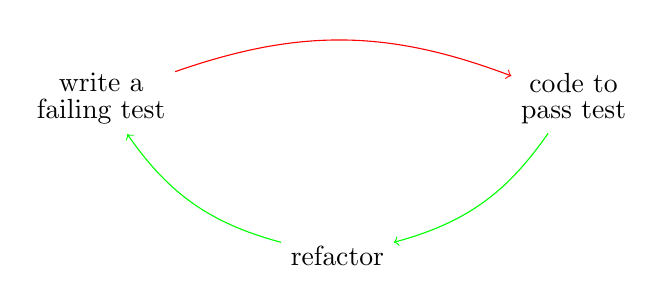
\begin{tikzpicture}[x=3cm]
                        \node (w) at (0, 0) {\shortstack{write a\\failing  test}};
                        \node (c) at (2, 0) {\shortstack{code to\\pass test}};
                        \node (r) at (1, -2) {refactor};
                        \draw
                        (w) edge[red, ->, bend left=20] (c)
                        (c) edge[green, ->, bend left=20] (r)
                        (r) edge[green, ->, bend left=20] (w);
                    \end{tikzpicture}
                \end{center}
                We start by writing failing tests, which seems counterintuitive, as there is no code to test.
                However, these tests are written as if the code was working - which gives us a specification on how the code \textbf{should} behave.
                We want to write code as quickly as possible that gets us from the \red{red} state (failing tests), to a \textcolor{green}{green} state (passing tests).
                This code is likely untidy - we can then tidy it up (which shouldn't break the tests).
                \medskip

                Additionally, it's not only about testing; we can replace the stages as follows;
                \begin{itemize}
                    \itemsep0em
                    \item API design \hfill (write a failing test)
                        \subitem "I wish there was a method that would take these parameters and do this"
                    \item internals design \hfill (code to pass test)
                        \subitem "Just making it work"
                    \item structural design \hfill (refactor)
                        \subitem "How can we improve the design?" (pyramid layers)
                \end{itemize}
                We focus more on what it should do (how it should behave), and not how it does it.
                For example, ~CustomerLookup~ should do the following;
                \begin{itemize}
                    \itemsep0em
                    \item finds customer by ID
                    \item fails for duplicate customers
                \end{itemize}
                The test is named as the expected result, and if it is true, then it behaves correctly.
                \begin{lstlisting}
                    public class CustomerLookupTest {
                      @Test
                      findsCustomerById() {
                        ...
                      }
                      @Test
                      failsForDuplicateCustomers() {
                        ...
                      }
                    }
                \end{lstlisting}
            \subsubsection*{Example of TDD}
                The object ~FibonacciSequence~ should do the following;
                \begin{itemize}
                    \itemsep0em
                    \item defines the first two terms to be one
                    \item has each term equal to the sum of the previous two
                    \item is not defined for negative terms
                \end{itemize}
                \begin{lstlisting}
                    ... // (FibonacciSequenceTest.java)

                    import static org.hamcrst.CoreMatchers.is;
                    import static org,junit.Assert.assertThat;

                    import org.junit.Test;

                    public class FibonacciSequenceTest {

                      @Test
                      public void definesFirstTwoTermsToBeOne() {
                        assertThat(new FibonacciSeqeunce().term(0), is(1));
                        assertThat(new FibonacciSeqeunce().term(1), is(1));
                      }
                    }
                \end{lstlisting}
                Obviously, none of this will work yet, as the code doesn't exist.
                However, we can use this to create the code as follows (this is incorrect, but our tests now pass);
                \begin{lstlisting}
                    ... // (FibonacciSequence.java)

                    public class FibonacciSequence {

                      public int term(int i) {
                        return 1;
                      }
                    }
                \end{lstlisting}
                We can then add more tests, which should now fail;
                \begin{lstlisting}
                    ... // (FibonacciSequenceTest.java)

                    public class FibonacciSequenceTest {
                      ...

                      @Test
                      public void hasEachTermTheSumOfPreviousTwo() {
                        assert(new FibonacciSeqeunce().term(2), is(2));
                        assert(new FibonacciSeqeunce().term(3), is(3));
                        assert(new FibonacciSeqeunce().term(4), is(5));
                      }
                    }
                \end{lstlisting}
                Similarly, we can modify the code again to add a naive implementation which performs it recursively;
                \begin{lstlisting}
                    ... // (FibonacciSequence.java)

                    public class FibonacciSequence {

                      public int term(int i) {
                        if (i < 2) {
                          return 1;
                        }
                        return term(i - 1) + term(i - 2);
                      }
                    }
                \end{lstlisting}
                Adding the last bullet point as a test;
                \begin{lstlisting}
                    ... // (FibonacciSequenceTest.java)

                    public class FibonacciSequenceTest {
                      ...

                      @Test
                      public void isNotDefinedForNegativeIndices() {
                        try {
                          new FibonacciSeqeunce().term(-1);
                          fail("should have thrown exception")
                        } catch (IllegalArgumentException iae) {
                          assertThat(iae.getMessage(), containsString("negative index"))
                        }
                      }
                    }
                \end{lstlisting}
                Fixing this, we add the following;
                \begin{lstlisting}
                    ... // (FibonacciSequence.java)

                    public class FibonacciSequence {

                      public int term(int i) {
                        if (i < 0) {
                          throw new IllegalArgumentException("negative index not supported");
                        }

                        ...
                      }
                    }
                \end{lstlisting}
                This is the only time I will actually write out every step, since that's the focus of TDD.
\end{document}
